\documentclass[pdftex,12pt,a4paper]{article}

\usepackage{graphicx}  
\usepackage[margin=2.5cm]{geometry}
\usepackage{breakcites}
\usepackage{indentfirst}
\usepackage{pgfgantt}
\usepackage{pdflscape}
\usepackage{float}
\usepackage{epsfig}
\usepackage{epstopdf}
\usepackage[cmex10]{amsmath}
\usepackage{stfloats}
\usepackage{multirow}

\renewcommand{\refname}{REFERENCES}
\linespread{1.3}

\usepackage{mathtools}
%\newcommand{\HRule}{\rule{\linewidth}{0.5mm}}
\thispagestyle{empty}
\begin{document}
\begin{titlepage}
\begin{center}
\textbf{}\\
\textbf{\Large{ISTANBUL TECHNICAL UNIVERSITY}}\\
\vspace{0.5cm}
\textbf{\Large{COMPUTER ENGINEERING DEPARTMENT}}\\
\vspace{4cm}
\textbf{\Large{BLG 222E\\ COMPUTER ORGANIZATION\\ PROJECT 1 REPORT}}\\
\vspace{4cm}
\begin{table}[ht]
\centering
\Large{
\begin{tabular}{lcl}
\textbf{CRN}  & : & 21335 \\
\textbf{LECTURER}  & : & Prof. Dr. Deniz Turgay Altılar \\
\end{tabular}}
\end{table}
\vspace{1cm}
\textbf{\Large{GROUP MEMBERS:}}\\
\begin{table}[ht]
\centering
\Large{
\begin{tabular}{rcl}
150220079  & : & AHMET ENES ÇİĞDEM \\
\end{tabular}}
\end{table}
\vspace{2.8cm}
\textbf{\Large{SPRING 2024}}

\end{center}

\end{titlepage}

\thispagestyle{empty}
\setcounter{tocdepth}{4}
\tableofcontents
\clearpage

\setcounter{page}{1}

\section{INTRODUCTION}

In our computer organization project, we constructed a basic computer system from fundamental components like the Instruction Register (IR), Register File, Address Register, and Arithmetic Logic Unit (ALU). By interconnecting these elements and integrating them with memory, we created a functional computational unit.

\section{MATERIALS AND METHODS}
We built all hardware part of this project by using Verilgo HDL via Xilinx Vivado.
\subsection{Part 1}
In this part, We implemented a basic register. This register has 8 functionalities that are controlled
by 3-bit control signals (FunSel) and an enable input (E). We will use this register in other part of this project.
\begin{figure}[htbp]
	\centering
	\includegraphics[width=0.7\textwidth]{Part 1 Image}
	\caption{Function table for part 1 register.}
\end{figure}

\subsection{Part 2}
(Part-2a)In this part, we designed a 16-bit IR register whose block diagram and function table are given
in Figure 2. This register can store 16-bit binary data. However, the input of this register
file is only 8 bits. Therefore, using the 8-bit input bus, you can load either the lower
(bits 7-0) or higher (bits 15-8) half. This decision is made by the L'H signal.
\begin{figure}[htbp]
	\centering
	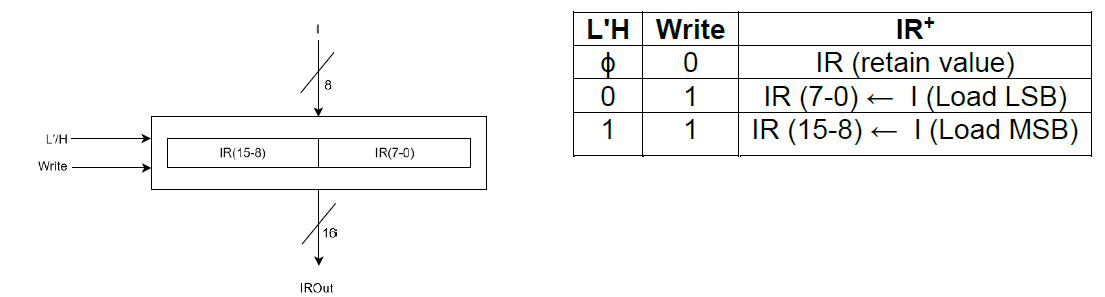
\includegraphics[width=0.7\textwidth]{Part 2.1 Image}
	\caption{Function table for instruction register.}
\end{figure} \par
(Part-2b)In this part, we design the system shown in Figure 3 which consists of four 16-bit general purpose registers: R1, R2, R3, R4, and four 16-bit scratch registers: S1, S2, S3, and S4. The details of inputs and outputs are as follows.
\begin{figure}[htbp]
	\centering
	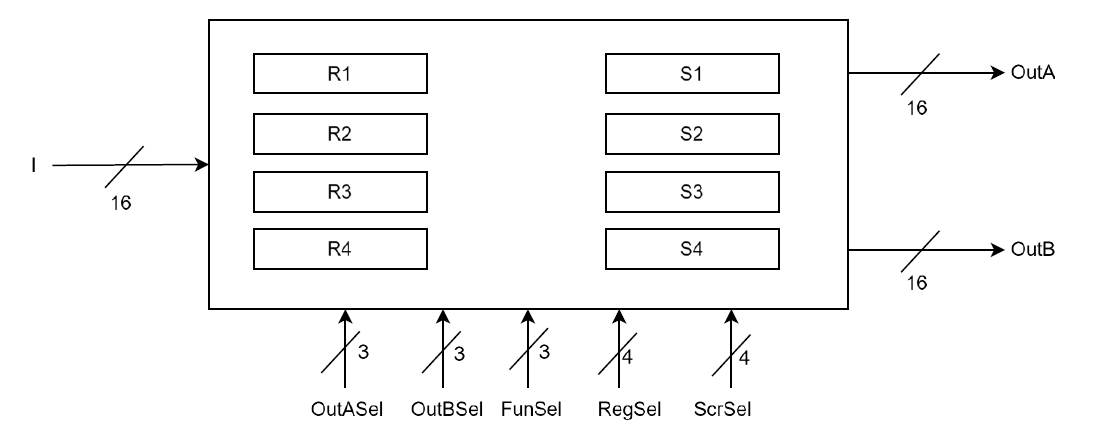
\includegraphics[width=0.7\textwidth]{Part 2.2 Image}
\end{figure} \par
OutASel and OutBSel are used to feed to output lines OutA and OutB, respectively. 16 bits of selected registers are output to OutA and OutB. Table 1 shows the selection of output registers based on the OutASel and OutBSel control inputs.
\begin{figure}[htbp]
	\centering
	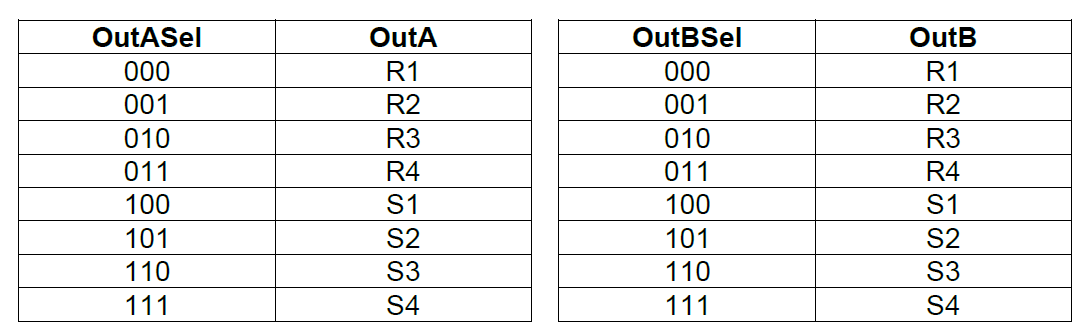
\includegraphics[width=0.7\textwidth]{Part 2 t1}
\end{figure} \par
RegSel and ScrSel are 4-bit signals that select the registers to apply the function that is determined by the 3-bit FunSel signal which is given in Table 2. The selected registers by RegSel and ScrSel are shown in Tables 3 and 4, respectively. \par
\begin{figure}[htbp]
	\centering
	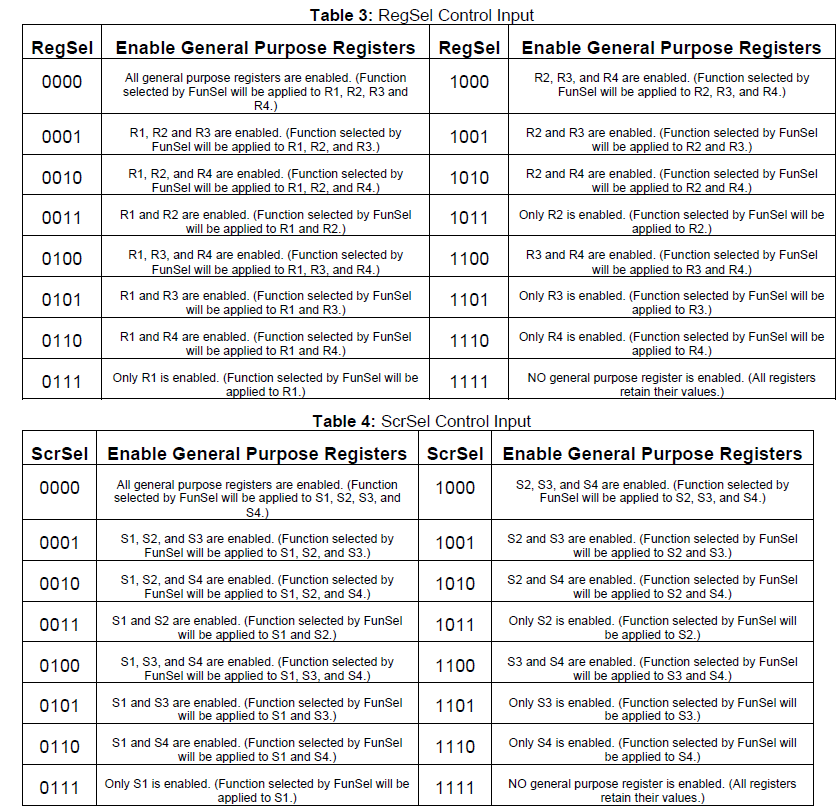
\includegraphics[width=0.7\textwidth]{Part 2 t3}
\end{figure}
\newpage
\begin{figure}[htbp]
	\centering
	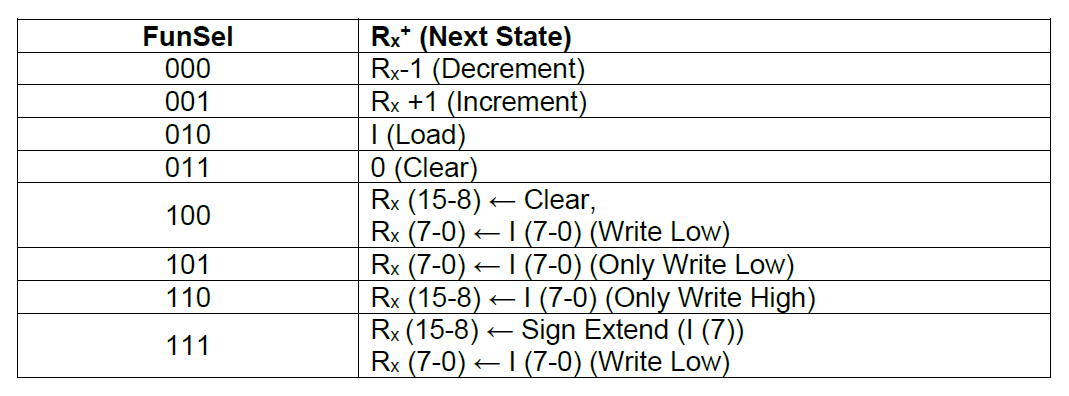
\includegraphics[width=0.7\textwidth]{Part 2 t2}
\end{figure} \par
\newpage
(Part-2c) In this part we design the address register file (ARF) system shown in Figure 4 which consists of three 16-bit address registers: program counter (PC), address register (AR), and stack pointer (SP). FunSel and RegSel work as in Part-2b. \par

\begin{figure}[htbp]
	\centering
	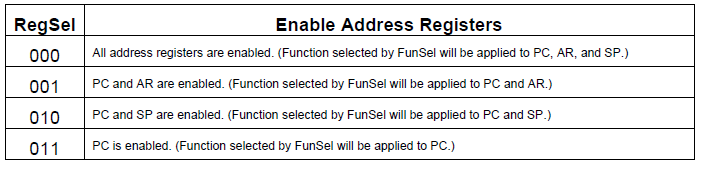
\includegraphics[width=0.7\textwidth]{Part 2.3 t1}
\end{figure} 
\begin{figure}[htbp]
	\centering
	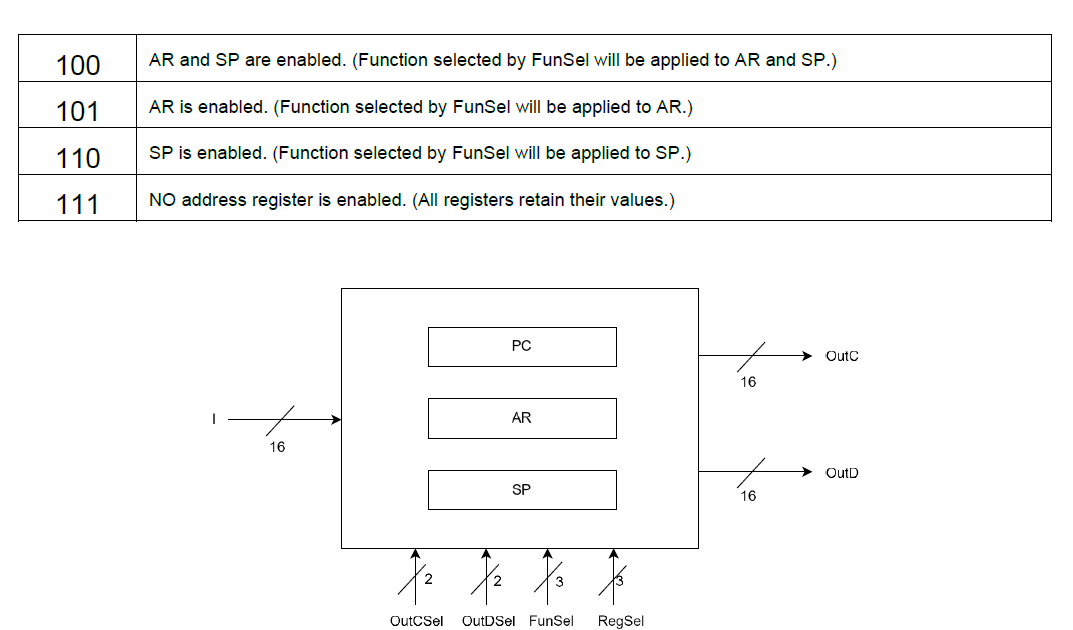
\includegraphics[width=0.7\textwidth]{Part 2.3 t2}
\end{figure} 
OutCSel and OutDSel are used to feed output lines OutC and OutD, respectively. 16 bits of the selected registers are output to OutC and OutD. Table below shows the selection of output registers based on the OutCSel and OutDSel control inputs.
\begin{figure}[H]
	\centering
	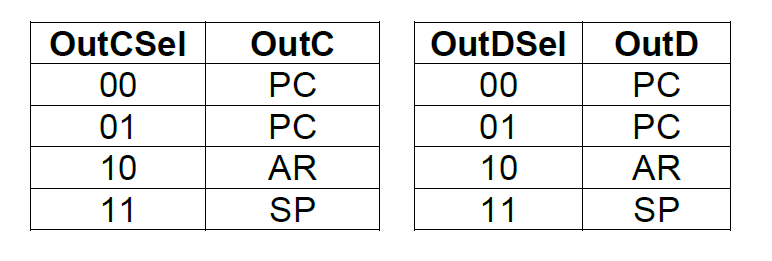
\includegraphics[width=0.7\textwidth]{Part 2.3 t3}
\end{figure} 

\subsection{Part 3}
(Part-3) In this part, we designed an Arithmetic Logic Unit (ALU) that has two 16-bit inputs, a 16-bit output, and a 4-bit output for zero, negative, carry, and overflow flags. The ALU is shown in Figure 5. The ALU functions and the flags that will be updated (i.e., - means that the flag will not be affected and + means that the flag changes based on the ALUOut) are given in Table below when WF (Write Flag) is 1.
\newpage 
\begin{itemize}
	\item FunSel selects the function of the ALU.
	\item ALUOut shows the result of the operation that is selected by FunSel and applied on A and/or B inputs.
	\item Arithmetic operations are done using 2’s complement logic.
	\item Z (zero) bit is set if ALUOut is zero (e.g. when NOT B is zero).
	\item C (carry) bit is set if ALUOut sets the carry (e.g. when LSL A produces carry)
	\item N (negative) bit is set if the ALU operation generates a negative result (e.g. when A-B results in a negative number).
	\item O (overflow) bit is set if an overflow occurs (e.g. when A+B results in an overflow).
	\item Note that Z|C|N|O flags are stored in a register! The Z flag is the MSB of the register, and the O flag is the LSB of the register.
\end{itemize}
\begin{figure}[htbp]
	\centering
	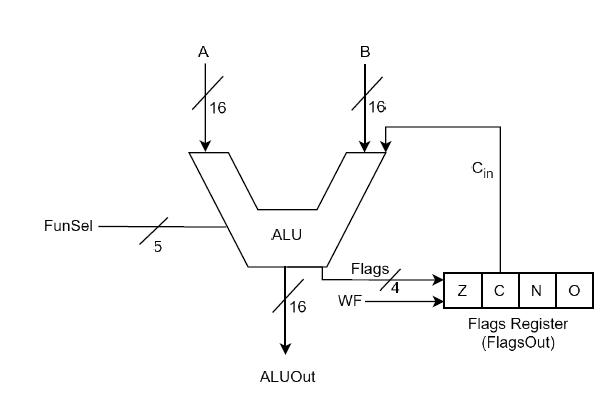
\includegraphics[width=0.7\textwidth]{Part 3 Image}
\end{figure}
\begin{figure}[H]
	\centering
	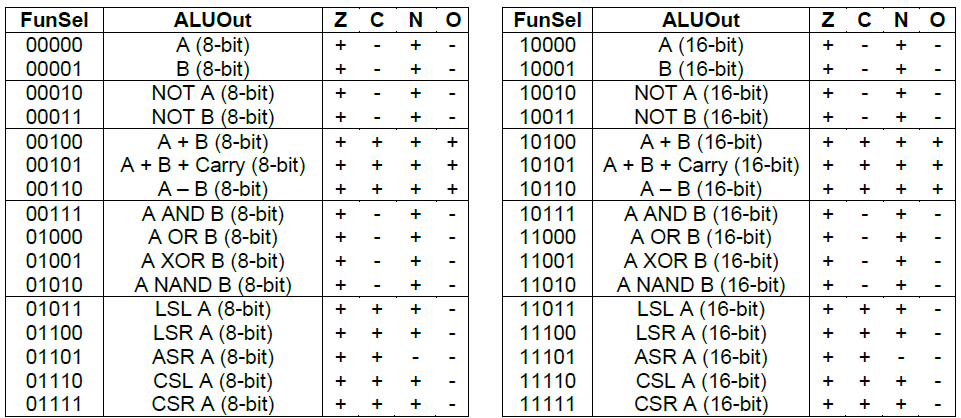
\includegraphics[width=1.0\textwidth]{Part 3 t1}
\end{figure}
\subsection{Part 4}
In this part we implemented the system that shown in the figure by using previous implementations.
\begin{figure}[htbp]
	\centering
	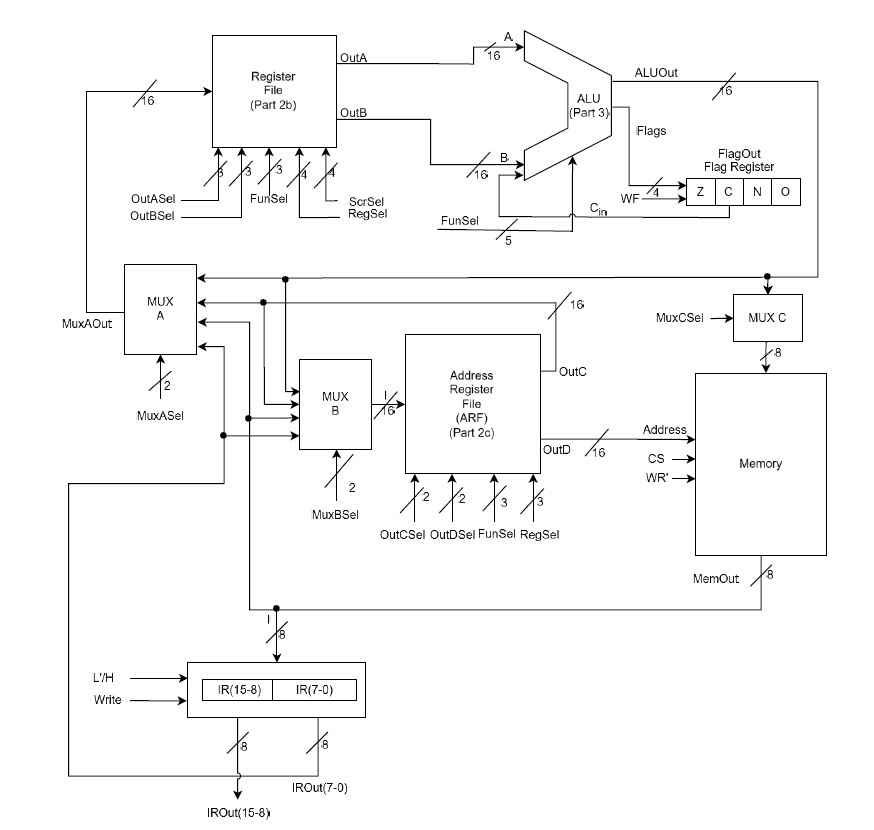
\includegraphics[width=0.8\textwidth]{Part 4 Image}
\end{figure}
\newpage
\section{RESULTS [15 points]}
We are given some simulation files. This part shows the results of this test files for each implementation.\par 
\subsection{Part 1}
Results of Register \par
\begin{figure}[H]
	\centering
	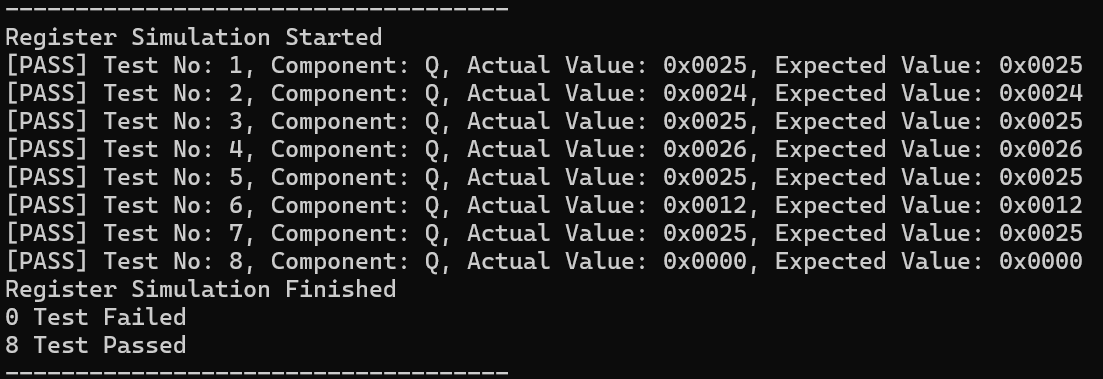
\includegraphics[width=0.7\textwidth]{R}
\end{figure}
\subsection{Part 2.1}
Results of Instruction Register \par
\begin{figure}[htbp]
	\centering
	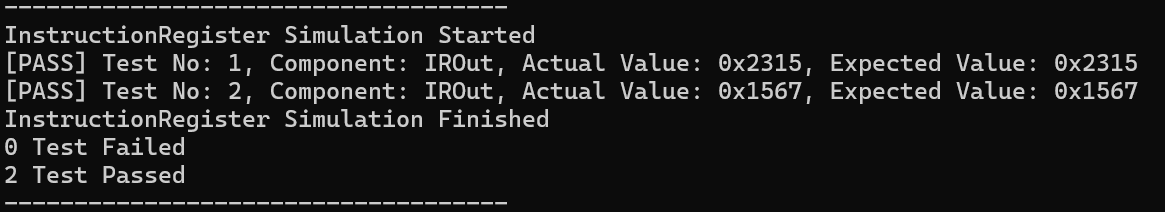
\includegraphics[width=0.7\textwidth]{IR}
\end{figure}
\subsection{Part 2.2}
Results of Register File \par
\begin{figure}[htbp]
	\centering
	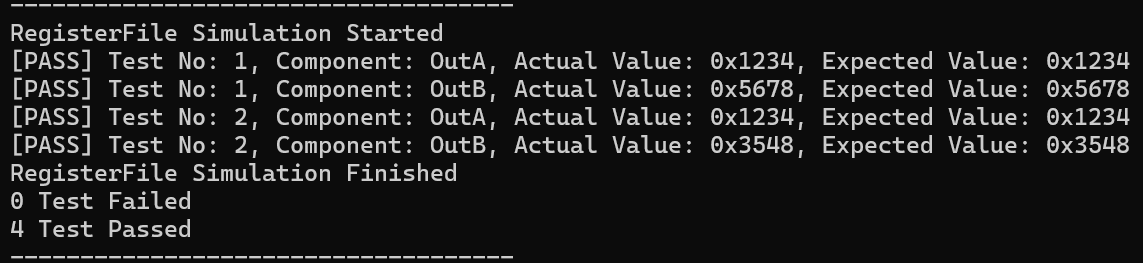
\includegraphics[width=0.7\textwidth]{RF}
\end{figure}
\newpage
\subsection{Part 2.3}
Results of Address Register File \par
\begin{figure}[htbp]
	\centering
	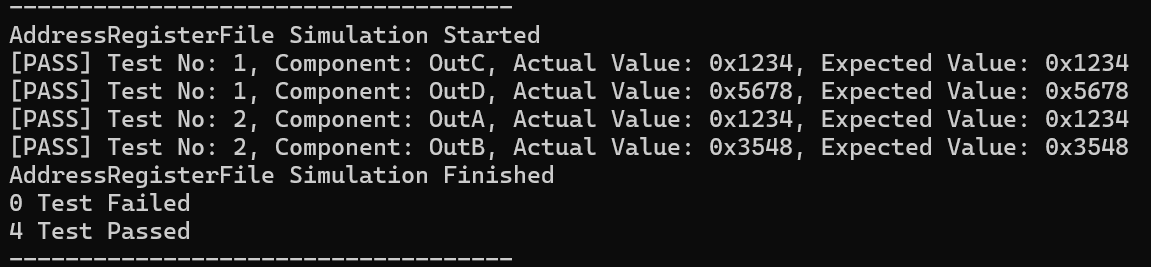
\includegraphics[width=0.7\textwidth]{ARF}
\end{figure}
\subsection{Part 3}
Results of Arithmetic Logic Unit \par
\begin{figure}[H]
	\centering
	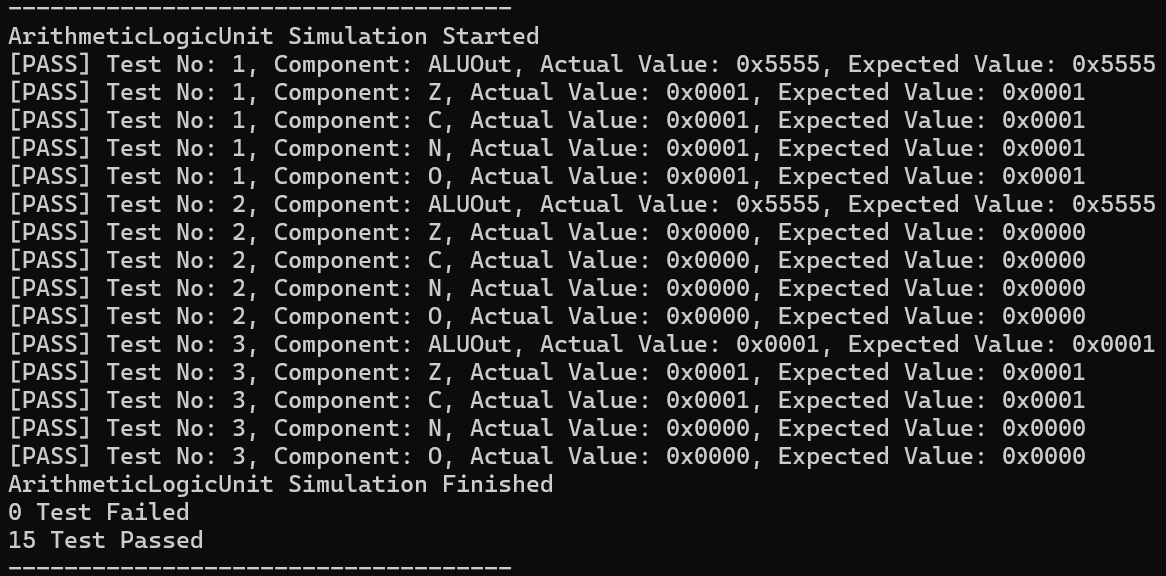
\includegraphics[width=0.7\textwidth]{ALU}
\end{figure}
\newpage
\subsection{Part 4}
Results of Arithmetic Logic Unit System \par
\begin{figure}[H]
	\centering
	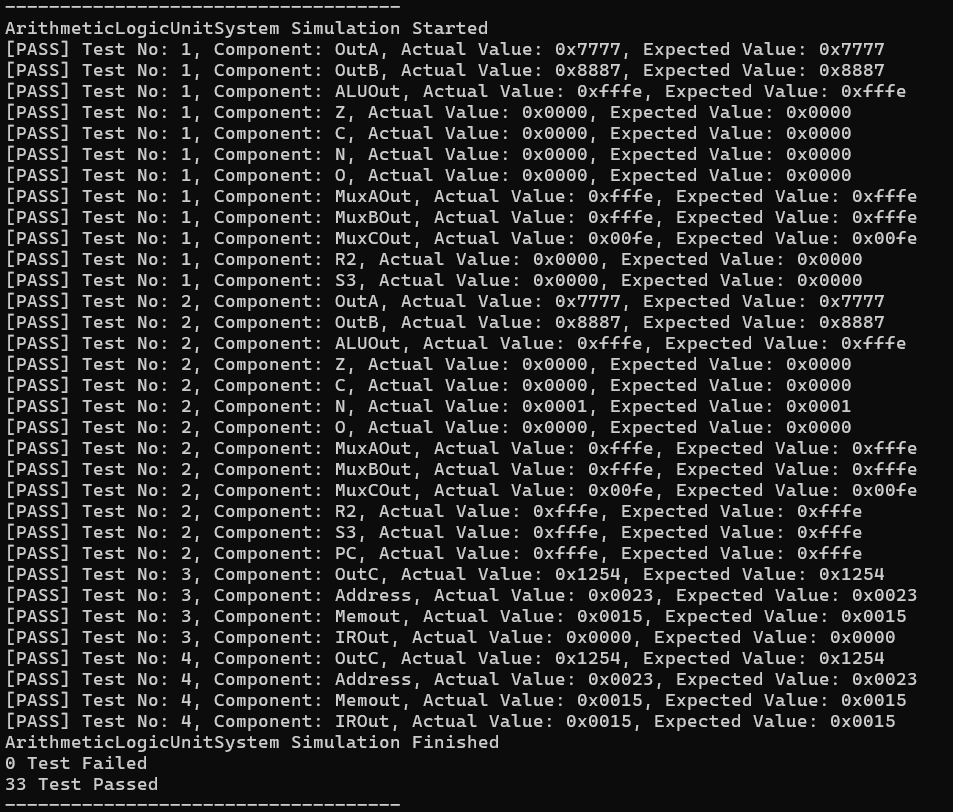
\includegraphics[width=0.7\textwidth]{ALUSys}
\end{figure}
\section{DISCUSSION}
\subsection{Part 1}
The project involves the design of a 16-bit register with versatile functionality controlled by 3-bit control signals (FunSel) and an enable input (E). The register's operation is determined by the combination of these control signals, allowing for eight distinct functionalities. The graphic symbol of the register, along with its characteristic table, facilitates understanding of its behavior. The register's flexibility and configurability make it a valuable component for subsequent stages of the project, enabling diverse operations within a digital system.
\newpage
\subsection{Part 2.1}
The project entails designing a 16-bit Instruction Register (IR) with specified block diagram and function table, as depicted in the report. The IR serves as a storage unit for 16-bit binary data. Notably, while the register has the capacity to store 16 bits, the input bus is only 8 bits wide. As a result, the register incorporates functionality to load either the lower half (bits 7-0) or the higher half (bits 15-8) of the input data, determined by the L'H signal. This capability allows for versatile usage of the IR within digital systems, facilitating efficient data storage and manipulation in accordance with system requirements.
\subsection{Part 2.2}
The project involves designing a system, comprising four 16-bit general-purpose registers (R1, R2, R3, R4) and four 16-bit scratch registers (S1, S2, S3, S4). The system incorporates two output lines, OutA and OutB, driven by control signals OutASel and OutBSel, respectively. Based on the values of OutASel and OutBSel, 16 bits of data from selected registers are output to OutA and OutB. The selection of output registers is determined by output selection table given above. Furthermore, the system includes control signals RegSel and ScrSel, both 4-bit signals, used to select registers for executing functions specified by the 3-bit FunSel signal. Tables for RegSel and ScrSel outline the registers selected by RegSel and ScrSel, respectively. This design facilitates flexible data storage, retrieval, and manipulation within the system, catering to diverse operational requirements.
\subsection{Part 2.3}
The part involves designing an Address Register File (ARF) system, comprising three 16-bit address registers: Program Counter (PC), Address Register (AR), and Stack Pointer (SP). The system operates with control signals FunSel and RegSel, akin to Part-2b. Additionally, the system incorporates control signals OutCSel and OutDSel, utilized to direct data to output lines OutC and OutD, respectively. 16 bits of data from selected registers are output to OutC and OutD based on the values of OutCSel and OutDSel. This design facilitates efficient management and manipulation of address data within the system, supporting diverse functionalities and operational requirements.
\subsection{Part 3}
The part entails designing an Arithmetic Logic Unit (ALU) featuring two 16-bit inputs, a 16-bit output, and a 4-bit output for zero, negative, carry, and overflow flags. The ALU's operation is governed by control signals (FunSel), determining various arithmetic and logical functions as detailed in Table given in the report. These functions include arithmetic operations conducted using 2’s complement logic, with corresponding flag updates stored in a register. The ALU's output provides essential data for subsequent processing within the system, contributing to efficient computation and decision-making.
\subsection{Part 4} 
In this part we implemented a design that includes all of previous implementation of this project. This part includes MuxA, MuxB and MuxC that enable us to manipulate corresponding inputs of each part thus, we can process some predetermined programs in the memory.

\section{CONCLUSION}
In conclusion, the design and implementation of the various components—ranging from the 16-bit register systems to the Arithmetic Logic Unit (ALU)—have culminated in a robust and versatile digital system. Each component, meticulously crafted to fulfill specific functional requirements, contributes to the overall functionality and efficiency of the system. The Address Register File (ARF) system facilitates seamless management and manipulation of address data, while the register systems provide essential storage capabilities. The ALU, with its array of arithmetic and logical functions, empowers the system with the ability to perform complex computations and decision-making tasks. Together, these components form a cohesive and adaptable digital system capable of executing a diverse range of operations, paving the way for further exploration and development in the realm of digital systems design.


\newpage
\addcontentsline{toc}{section}{\numberline {}REFERENCES}

\bibliographystyle{unsrt}
\bibliography{reference}

\end{document}

